\chapter{Metodologia}
\label{chap:metodologia}

\section{Southern Photometric Local Universe Survey (S-PLUS)}
\label{sec:splus}

Os grandes levantamentos (\emph{surveys}), sejam eles espectroscópicos ou fotométricos, são muito importantes para nossa compreensão do universo. Esses levantamentos mapeiam a distribuição tridimensional de galáxias, aglomerados de galáxias e outras estruturas em largas escalas, de forma a ilustrar como o universo é organizado e como essas estruturas evoluíram ao longo do tempo. Ao examinar o espectro de luz de galáxias distantes, os \emph{surveys} espectroscópicos revelam informações valiosas sobre a história, evolução e expansão do universo, investigando a natureza da matéria escura e da energia escura, dois dos maiores desafios da física e da cosmologia modernas. Os levantamentos fotométricos fornecem informações detalhadas sobre a distribuição espacial, tamanho, forma, cor e luminosidade das galáxias. Isso é fundamental para investigar como as galáxias se formaram, evoluíram e se enriqueceram ao longo do tempo e como interagem umas com as outras em diferentes ambientes. A fotometria de alta precisão é essencial, por exemplo, na detecção e caracterização de exoplanetas (planetas fora do nosso sistema solar). Ambos os tipos de levantamentos desempenham um papel importante na astronomia, astrofísica e cosmologia, fornecendo dados para testar modelos teóricos e investigar fenômenos. 

\subsection{Instrumentação e ciência}

Nesta pesquisa, trabalhamos com os dados fotométricos do Southern Photometric Local Universe Survey (S-PLUS)\footnote{Mais informações em: https://www.splus.iag.usp.br.} para estudar galáxias peculiares aneladas do hemisfério sul do universo local. O S-PLUS é um levantamento por imagem que cobrirá aproximadamente 8000 $\mathrm{graus}^{2}$ do céu do hemisfério sul em altas latitudes galácticas e cerca de 1300 $\mathrm{graus}^{2}$ sobre o disco e o bojo de nossa galáxia ao final do lançamento de seus dados, e utiliza um telescópio robótico (T80S) de abertura de 0,8 metros no Observatório Interamericano Cerro Tololo (CTIO), no Chile. O projeto S-PLUS, possui colaboração internacional fundada pela Universidade de São Paulo, Observatório Nacional, Universidade Federal de Sergipe, Universidad de La Serena e Universidade Federal de Santa Catarina. Ele possui um sistema de 12 filtros, combinados em 5 bandas largas similares ao SDSS (Sloan Digital Sky Survey), $u$, $g$, $r$, $i$ e $z$, sendo que o filtro de banda $u$ é o filtro de \emph{Javalambre} e possui uma curva de transmissão mais eficiente comparada com a banda $u$ do SDSS, conforme descreve \citeonline{2019A&A...622A.176C}, e 7 bandas estreitas centradas em linhas de absorção e emissão específicas, importantes para caracterização da distribuição espectral de energias em classificação de estrelas, $[\text{OII}]$, Ca H+K, banda G, H$\delta$, tripleto de Mgb, H$\alpha$ e tripleto de Ca (mais informações em \citeonline{2019MNRAS.489..241M}). O telescópio possui a câmera T80Cam-S e o detector (CCD) de matriz de 9232 × 9216 pixels, com uma escala de 0,55'' $\mathrm{pixel}^{-1}$ (segundos de arco por pixel) e um campo de visão (\emph{field of view}, FoV) de 1,4 × 1,4 graus.

\begin{figure}[h]
  \centering 
  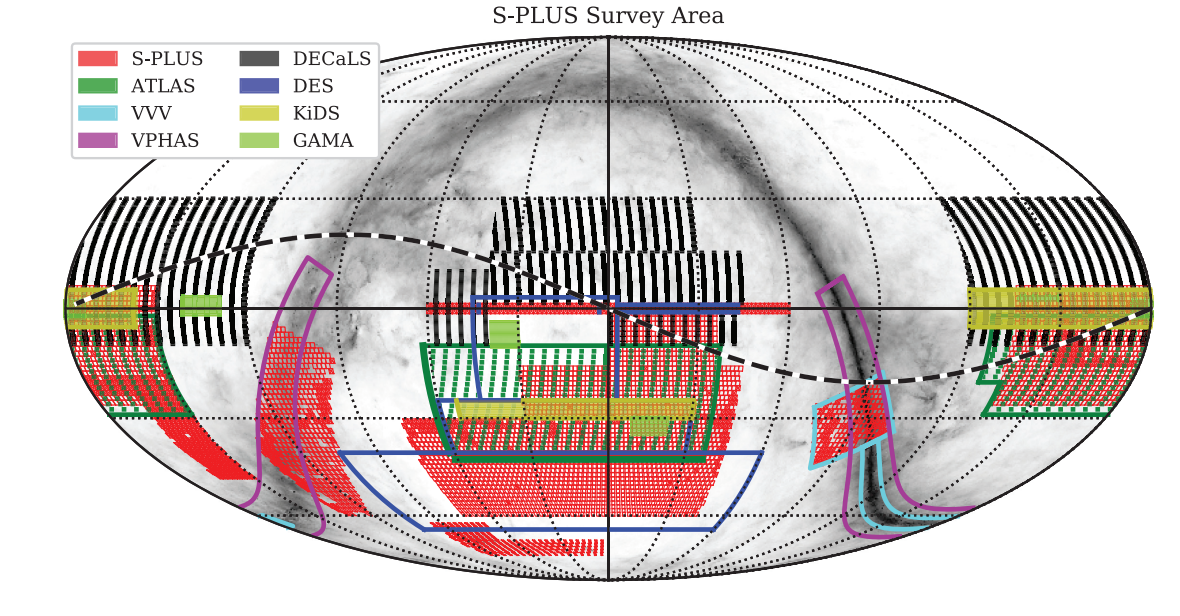
\includegraphics[width=0.9\textwidth]{Imagens/surveyarea.PNG} 
  \caption[Área de cobertura do S-PLUS.]{Em vermelho, a área de cobertura do S-PLUS, comparada a alguns levantamentos ópticos e de infravermelho próximo no hemisfério sul. Créditos: \citeonline{2019MNRAS.489..241M}.}
  \label{fig:surveyarea} 
\end{figure}

\begin{figure}[h]
  \centering 
  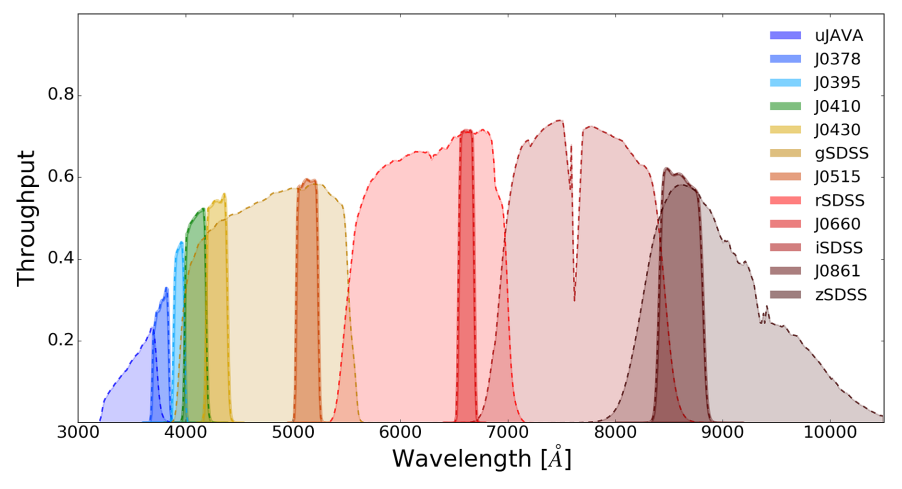
\includegraphics[width=0.8\textwidth]{Imagens/dozefiltros.PNG} 
  \caption[Sistema de 12 filtros do S-PLUS.]{A imagem mostra a eficiência total dos filtros em função do comprimento de onda. Diferentes cores são representadas para cada filtro de acordo com a legenda à direita. Os filtros J0378, J0395, J0410, J0430, J0515, J0660 e J0861 são, respectivamente, $[\text{OII}]$, Ca H+K, H$\delta$, banda G, tripleto de Mgb, H$\alpha$ e tripleto de Ca. Créditos: \citeonline{2019MNRAS.489..241M}.}
  \label{fig:dozefiltros} 
\end{figure}

\begin{figure}[h]
  \centering 
  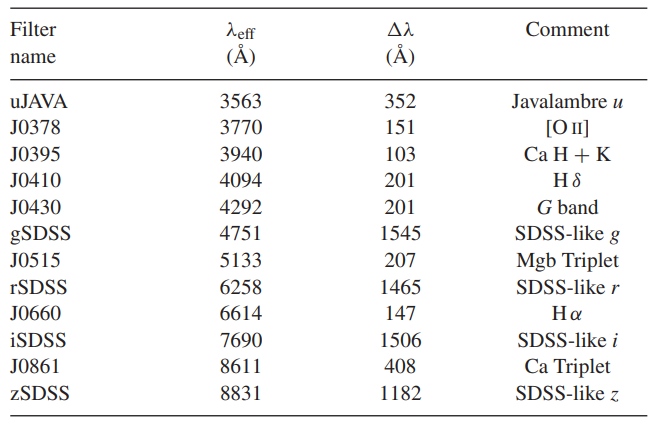
\includegraphics[width=0.7\textwidth]{Imagens/filtros.PNG} 
  \caption[Sumário dos filtros do S-PLUS.]{A tabela mostra as especificações dos comprimentos de onda centrais de cada filtro e a largura total à meia altura (FWHM\footnotemark) das curvas de transmissão. Créditos: \citeonline{2019MNRAS.489..241M}.}
  \label{fig:filtros} 
\end{figure}
\footnotetext{Do inglês, \emph{Full Width at Half Maximum} (Largura Total à Meia Altura), é uma medida de largura de um pico de distribuição que indica o intervalo entre os pontos em que a função tem metade do seu valor máximo.}

Uma das importantes vantagens do S-PLUS é o seu nível de resolução somado ao sistema de bandas estreitas para extrair informações para uma grande quantidade de objetos. Ele fornecerá uma precisão de \emph{redshift} fotométrico z = 0.02 (ou melhor) para galáxias com r < 19.7 mag AB ou z < 0.4, e para galáxias com r < 21 mag AB ou z < 0.5, precisão de z = 0.03, grande mapeamento 3D do universo local (\citeonline{2019MNRAS.489..241M}; \citeonline{2022MNRAS.511.4590A}). O \emph{redshift} fotométrico é uma técnica utilizada na astronomia para estimar o desvio para o vermelho (z) de objetos astronômicos com base em suas características espectrais capturadas em imagens fotométricas, uma maneira rápida e eficiente (em termos de tempo de observação) de estimar \emph{redshift}\footnote{O redshift descreve o deslocamento das linhas espectrais de um objeto em direção ao espectro do vermelho. Esse desvio para o vermelho é uma medida do quão longe e quão rápido um objeto se afasta de nós no espaço (ou blueshift, deslocamento das linhas espectrais de um objeto em direção ao espectro do azul, e ocorre quando o objeto está se aproximando do observador), bem como à expansão do Universo.} para um grande número de objetos, e com isso, estudar a velocidade, direção do movimento e distribuição espacial de galáxias, evolução do universo, determinar distâncias e outras ciências.

Os dados\footnote{Documentação do banco de dados disponível em: https://splus.cloud.} do catálogo fotométrico multi-banda incluem as magnitudes medidas em seis aberturas diferentes para cada filtro, geradas executando o software SExtractor\footnote{Documentação: https://sextractor.readthedocs.io/en/latest/index.html.} (\citeonline{1996A&AS..117..393B}; \citeonline{2010ascl.soft10064B}): aberturas elípticas variáveis (auto e petro), abertura isofotal (iso), aberturas aper 3 e aper 6 circulares fixas e a abertura circular PStotal. O SExtractor, inicialmente, realiza a análise de uma imagem de forma automatizada e calcula uma estimativa do nível de fundo em qualquer posição da imagem (mapa de fundo). O modelo do fundo do céu é construído e computadas as estatísticas. Os pixels da imagem são subtraídos desse fundo, filtrados e as detecções são limpas e medidas. As imagens finais e astrometricamente corrigidas, são geradas como uma combinação de exposições individuais de cada filtro usando, respectivamente, o SExtractor \cite{2010ascl.soft10064B} e o PSFEx \cite{2013ascl.soft01001B}, SCAMP \cite{2010ascl.soft10063B} e SWARP \cite{2010ascl.soft10068B}. Por fim, as medidas são escritas no catálogo de saída. As medições são feitas nos contornos isofotais dos objetos, definidos na imagem de detecção filtrada. Somente pixels com valores acima do limiar de detecção (fundo) são considerados e constituem o contorno isofotal, e o software opera neles os parâmetros (denominados de \emph{primeiro momento}) para definir as aberturas elípticas: as coordenadas do baricentro (x e y), indica a posição do ``centro'' de uma fonte; formatos básicos elípticos (eixo maior A, eixo menor B e ângulo de inclinação Theta) para representar a dispersão espacial máxima e mínima do perfil do objeto ao longo de qualquer direção; e elongação e elipticidade (parâmetros de elipse derivados de A e B). As magnitudes das aberturas, expressas no sistema AB (Absolute AB), e todos os valores dos parâmetros para cada fonte detectada são fornecidos pelo S-PLUS. Nesta pesquisa, analisamos as aberturas elípticas variáveis auto, petro e a abertura isofotal para o estudo das galáxias peculiares aneladas.

\begin{figure}[h]
  \centering 
  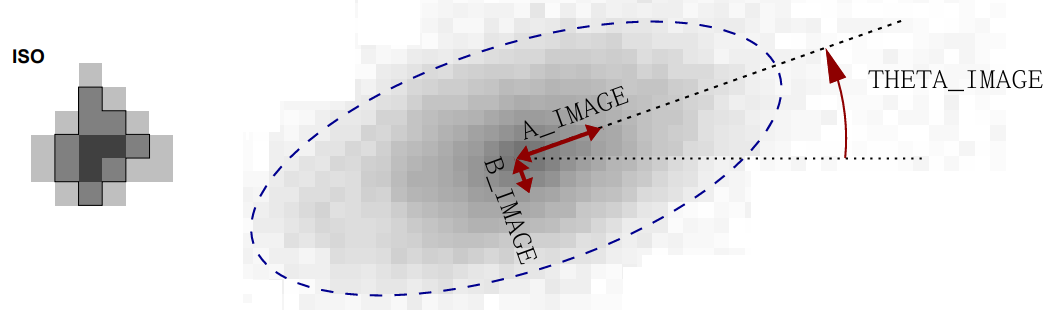
\includegraphics[width=0.8\textwidth]{Imagens/iso_elipse.png} 
  \caption[Detecção de uma fonte e parâmetros da elipse.]{Exemplo de uma detecção de pixels com valores acima do limiar (iso) e os parâmetros de formatos básicos de uma elipse computados em seguida.}
  \label{fig:iso_elipse} 
\end{figure}

\subsection{Abertura ISO}
Iso: A partir das medições do \emph{primeiro momento} (x, y, A, B, theta, elongação e elipticidade) feitas nos contornos isofotais das detecções, um parâmetro escalar (equação \ref{eq:parametro_escalar}), é computado para dimensionar a elipse, denominado de R, baseado em CXX, CYY e CXY (baricentros que também representam a mesma elipse). Desta forma, a área isofotal total é obtida para cada fonte.
\newcommand{\CXX}{C_{\text{XX}}}
\newcommand{\CYY}{C_{\text{YY}}}
\newcommand{\CXY}{C_{\text{XY}}}
\begin{equation} \label{eq:parametro_escalar}
\large
\CXX(x-\bar{x})^2 + \CYY(y-\bar{y})^2 + \CXY(x-\bar{x})(y-\bar{y}) = R^2
\end{equation}

Geralmente, o limite isofotal de um objeto detectado é bem representado por $R \approx 3$, mas para fontes estendidas esse parâmetro varia. O fluxo ISO para cada filtro é determinado pela equação \ref{eq:fluxo_iso}, onde \emph{pi} são os pixels detectados acima do fundo e \emph{S} a distribuição espacial dos pixels:
\begin{equation} \label{eq:fluxo_iso}
\large
\text{Fluxo}_{(iso)} = \sum_{i \in S} pi
\end{equation}

\begin{figure}[h]
  \centering 
  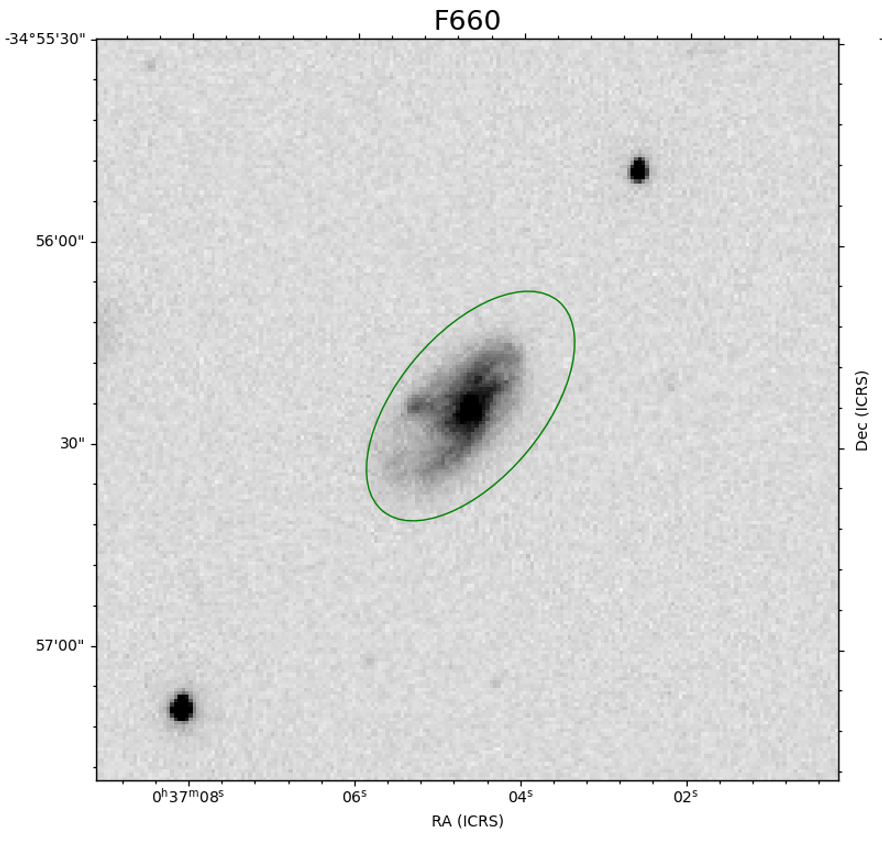
\includegraphics[width=0.6\textwidth]{Imagens/iso_exemplo.png} 
  \caption[Exemplo da abertura ISO para a galáxia AM 0034-351.]{Exemplo da abertura ISO computada usando o SExtractor pelo S-PLUS para a galáxia peculiar anelada AM 0034-351.}
  \label{fig:iso_exemplo} 
\end{figure}

\subsection{Abertura elíptica variável AUTO}
Auto: Definida em termos do raio de \citeonline{1980ApJS...43..305K} e obtida a partir das medições do \emph{primeiro momento} (x, y, A, B, theta, elongação e elipticidade) feitas nos contornos isofotais das detecções. Os eixos A e B da elipse são multiplicados por 6 (o que corresponde aproximadamente a duas vezes o tamanho do contorno isofotal em cada eixo). O fator de Kron (raio de Kron) é calculado dentro dessa abertura elíptica pela equação \ref{eq:kron_radius} e a elipse de Kron (abertura auto) determinada, onde \emph{pi} são os pixels na imagem de detecção acima do fundo, \emph{ri} é o ``pseudo-raio reduzido'' no pixel \emph{i} e \emph{E} a abertura elíptica.
\begin{equation} \label{eq:kron_radius}
\scalebox{1.4}{$\displaystyle \frac{\sum_{i \in \mathit{E}} ri \, pi}{\sum_{i \in \mathit{E}} pi}$}
\end{equation}

A abertura elíptica de Kron (abertura auto) é a elipse com o raio de Kron aplicado ao \emph{primeiro momento} do algoritmo. Objetos com muito ruído podem acabar com uma elipse de Kron pequena, desta forma, o SExtractor impõe um tamanho mínimo para o raio de Kron para 2.0 e máximo de 3.5. O S-PLUS alterou os parâmetros para 1.82 e 3.00 para melhor representar a magnitude total das fontes. Após a abertura elíptica auto gerada, o fluxo das fontes para cada filtro é calculado pela soma dos valores dos pixels em unidas de AB mag pela equação \ref{eq:kron_flux}, onde \emph{K} é a abertura elíptica de Kron.
\begin{equation} \label{eq:kron_flux}
\large
\text{Fluxo}_{(auto)} = \sum_{i \in K} pi
\end{equation}

\begin{figure}[h]
  \centering 
  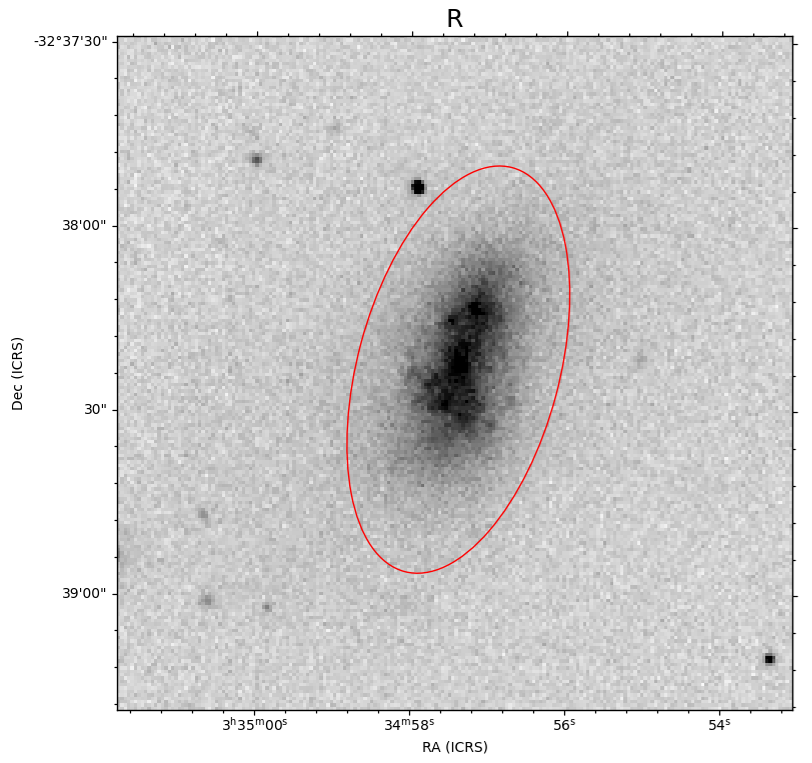
\includegraphics[width=0.6\textwidth]{Imagens/auto_exemplo.png} 
  \caption[Exemplo da abertura AUTO para a galáxia AM 0332-324.]{Exemplo da abertura AUTO em termos do raio de Kron computada usando o SExtractor pelo S-PLUS para a galáxia peculiar anelada AM 0332-324.}
  \label{fig:auto_exemplo} 
\end{figure}

\subsection{Abertura elíptica variável PETRO}
Petro: Similar à abertura auto, a abertura elíptica variável petro é definida em termos do raio de \citeonline{1976ApJ...209L...1P}. Uma vez obtida as medições do \emph{primeiro momento} (x, y, A, B, theta, elongação e elipticidade) feitas nos contornos isofotais das detecções, os eixos A e B da elipse também são multiplicados por 6 e o fator de Petrosian (raio de Petrosian) é calculado dentro dessa abertura elíptica pela equação \ref{eq:petro_radius} e a elipse de Petro (abertura petro) determinada, onde \emph{pi} são os pixels na imagem de detecção acima do fundo e \emph{ri} é o ``pseudo-raio reduzido'' no pixel \emph{i}.
\begin{equation} \label{eq:petro_radius}
\scalebox{1.4}{$\displaystyle \left(\frac{\sum_{0.9r<ri<1.1r} p_i}{\sum_{ri<r} p_i}\right) \cdot \left(\frac{N_{\underset{ri<r}{\ }}}{N_{\underset{0.9r<ri<1.1r}{\ }}}\right)$}
\end{equation}

A abertura elíptica de Petrosian (abertura petro) é a elipse com o raio de Petrosian aplicado ao \emph{primeiro momento} do algoritmo. Da mesma forma que a abertura auto, o SExtractor impõe um tamanho mínimo para o raio de Petrosian para 2.0 e máximo de 3.5. O S-PLUS alterou os parâmetros para 2.0 e 2.73, respectivamente. Após a abertura elíptica petro gerada, o fluxo das fontes para cada filtro é calculado pela soma dos valores dos pixels, em unidas de AB mag, pela equação \ref{eq:petro_flux}, onde \emph{P} é a abertura elíptica de Petrosian e \emph{pi} são os pixels detectados acima do fundo. 
\begin{equation} \label{eq:petro_flux}
\large
\text{Fluxo}_{(petro)} = \sum_{i \in P} pi
\end{equation}

\begin{figure}[h]
  \centering 
  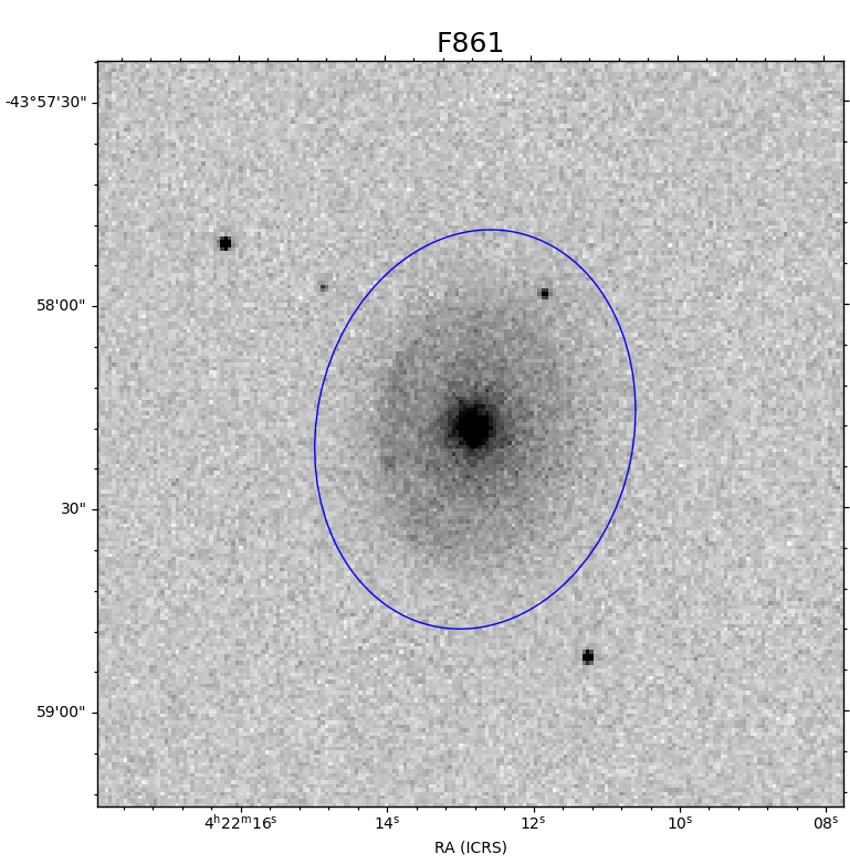
\includegraphics[width=0.6\textwidth]{Imagens/petro_exemplo.PNG} 
  \caption[Exemplo da abertura PETRO para a galáxia AM 0420-440.]{Exemplo da abertura PETRO em termos do raio de Petrosian computada usando o SExtractor pelo S-PLUS para a galáxia peculiar anelada AM 0420-440.}
  \label{fig:petro_exemplo} 
\end{figure}

Todos os parâmetros computados possuem seus respectivos erros estimados e são fornecidos pelo S-PLUS para cada filtro e abertura. O S/N\footnote{A relação sinal-ruído (S/N) avalia a confiabilidade e a precisão das medições de fluxo luminoso ou de intensidade de um objeto em relação ao ruído de fundo associado a ele.} é definido como o fluxo dividido pelo seu erro e para a não detecção em um determinado filtro, a magnitude é substituída por 99.

\section{Dados da amostra}

Inicialmente, as amostras foram selecionadas a partir de catálogos e atlas especializados em galáxias aneladas:

\begin{itemize}
    \item A catalogue of southern peculiar galaxies and associations de \citeonline{1987arpmadore} lista galáxias na Categoria 6, classificadas com anel bem definido ao redor e quaisquer galáxias morfologicamente parecidas. Os autores fazem uma breve descrição para cada objeto enfatizando aspectos como a direção de um jato ou o número de companheiros aparentes, etc. Todas as galáxias listadas na Categoria 6 foram consideradas neste estudo.
    \item New observations and a photographic atlas of polar-ring galaxies de \citeonline{1990AJ....100.1489W}, possui 157 galáxias divididas em quatro categorias: com anéis polares confirmados cinematicamente (categoria A), bons candidatos com base em sua aparência morfológica (categoria B), possíveis candidatos (categoria C) e objetos possivelmente relacionados (categoria D). Apenas as categorias A e B foram consideradas nesta pesquisa.
    \item A new catalogue of polar-ring galaxies selected from the Sloan Digital Sky Survey (SDSS) de \citeonline{2011MNRAS.418..244M}, possui 275 objetos classificados como galáxias peculiares com anel polar conforme imagens do SDSS. Este catálogo complementa o de \citeonline{1990AJ....100.1489W} e é baseado nos resultados do projeto Galaxy Zoo. As galáxias de anel polar foram divididas em quatro categorias pelos autores: melhores candidatas, boas candidatas, objetos relacionados a anel polar e anéis muito inclinados à linha de visão (\emph{face on} - vistos quase de frente). Para esta pesquisa, foram considerados apenas os melhores candidatos, bons candidatos e \emph{face on}.
    \item Atlas and catalog of collisional ring galaxies de \citeonline{2009ApJS..181..572M}, que extraíram  as galáxias de \citeonline{1987arpmadore} (onde listam na tabela 1) e complementaram com outras RGs conhecidas da literatura (tabela 2). Este trabalho lista a galáxia alvo e apresenta as posições plausíveis para os possíveis colisores companheiros próximos. Foram considerados apenas os objetos da tabela 2, visto que já tínhamos as informações da tabela 1 por referência do catálogo de \citeonline{1987arpmadore}. 
    \item Ring galaxies I, onde \citeonline{1976ApJ...208..650T} proporam um esquema de classificação para RGs, em três subclasses: galáxias RE de anéis vazios nítidos; galáxias RN, semelhantes às REs, mas com núcleo descentralizado; e galáxias RK, com nódulos ou condensações dominantes em seus anéis. Utilizaram observações fotométricas e espectroscópicas para estimar propriedades globais das RGs. Deste estudo, foram consideradas 10 galáxias, visto que as outras já faziam parte dos catálogos e atlas anteriores pesquisados.
    \item Search for faint ring-shaped galaxies in the -77 deg to -87 deg declination interval de \citeonline{1994A&AS..104....1F}. Os autores classificam os objetos candidatos a RGs de acordo com a estrutura do anel e a aparência do núcleo. Para nosso critério de amostras peculiares aneladas, foram considerados apenas os objetos classificados com anel tipo spher (esfera), ellip (elipse) e spindle (fuso ou estrutura alongada) pelos autores.
    \item The visual appearance of the nuclei of ring-shaped galaxies as an alternative classification criterion de \citeonline{1992A&AS...94..245F}, classifica prováveis RGs em relação à morfologia do núcleo. Consideramos para nossa lista apenas os objetos classificados pelos autores com anel tipo spher (esfera), ellip (elipse) e spindle (fuso ou estrutura alongada).
    \item On the morphology of peculiar ring galaxies, onde \citeonline{1998abans} dividiram as RGs em cinco tipos principais de acordo com a morfologia do anel e do bojo, com base na inspeção visual de objetos selecionados. Todos os objetos listados deste trabalho foram considerados para nosso estudo.
\end{itemize}

Uma lista inicial\footnote{Para visualização da lista, entrar em contato por e-mail: barbaralunarti@gmail.com.} foi criada com todas as galáxias referente aos catálogos e atlas citados acima, com os critérios descritos, e foram divididas em dois grupos distintos: as peculiares e as normais, seguindo rigorosamente as classificações previamente estabelecidas pelos trabalhos dos autores consultados. Em seguida, somente os objetos peculiares foram selecionados e atualizadas suas informações de RA (Right Ascension)\footnote{Ascensão reta: medida ao longo do equador celeste, partindo do ponto vernal (ponto de início do equador celeste) em direção ao leste, usada para indicar a posição leste-oeste de um objeto no céu.} e DEC (Declination)\footnote{Declinação: medida perpendicularmente ao equador celeste, indo de -90° (sul celeste) a +90° (norte celeste), usada para indicar a posição norte-sul de um objeto no céu.}, de acordo com os bancos de dados NASA/IPAC Extragalactic Database e SIMBAD Astronomical Database. As galáxias com nomes iguais (repetidas) foram removidas desta lista.

Em seguida, fizemos uma busca no banco de dados do S-PLUS para filtrar os objetos encontrados. Essa busca é através da Astronomical Data Query Language (ADQL), para realizar consultas astronômicas no banco de dados utilizando a linguagem de programação Python. A ADQL é baseada na Linguagem de Consulta Estruturada (SQL, do inglês Structured Query Language), usada para gerenciar dados em bancos de dados relacionais. A partir de nossa lista de objetos e suas respectivas coordenadas RA e DEC, filtramos as galáxias encontradas no S-PLUS até a última atualização de dados disponíveis (data releases 1, 2, 3 e 4). Uma segunda inspeção individual às nossas amostras foi realizada retirando objetos listados com um nome por um catálogo, sendo o mesmo, porém com designação diferente, por outro catálogo (Exemplo: por ordem de construção de nossa lista em relação aos catálogos e atlas consultados, o objeto FM 351-12 de \citeonline{1998abans} foi removido porque corresponde à AM 0053-353 do catálogo de \citeonline{1987arpmadore}). Os objetos classificados como galáxias espirais em transição ou nebulosas planetárias, de acordo com os bancos de dados NASA/IPAC Extragalactic Database e SIMBAD Astronomical Databasede, também foram removidos de nossa lista. Por fim, nossa lista primordial (Tabela \ref{tab:splus} - Apêndice A) para o estudo da fotometria de galáxias aneladas encontradas no S-PLUS possui apenas galáxias classificadas como peculiares conforme autores consultados, não há objetos repetidos mesmo com nomes diferentes e as coordenadas celestes foram atualizadas, totalizando 116 objetos.

As imagens\footnote{Imagens e informações dos dados utilizados: https://github.com/barbaralunarti.} por banda e a combinação dos 12 filtros (dois exemplos são as Figuras \ref{fig:filtroscartwheel} e \ref{fig:am0417391}) foram adquiridas através da função conecção \texttt{splusdata.connect}, onde a busca se faz pelas coordenadas RA e DEC do objeto de desejo. Para esta busca, também, pode-se aderir as preferências de filtros, isolados ou combinados, e o tamanho da imagem. Foram realizadas quatro buscas ADQL para obter: as imagens (no formato \emph{FITS Figure}) por filtro em escala preto e branco e os dados dos parâmetros das tabelas para gerar as elipses; os dados das magnitudes para cada filtro e seus respectivos erros, para as aberturas iso, auto e petro (separadamente), comparando os valores e as propriedades dos objetos. Plotamos as três aberturas elípticas conforme dados obtidos das tabelas e analisamos a fotometria em cada filtro de nossa amostra.